\section{Burn Notice}

\begin{wrapfigure}{rt}{.3\textwidth}
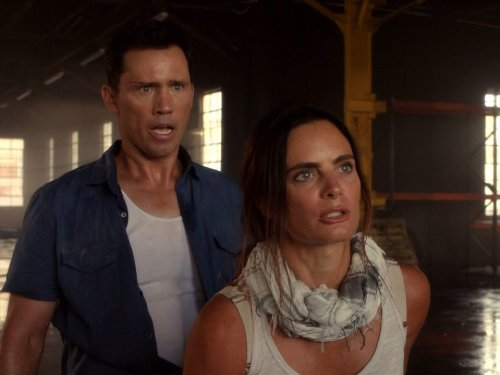
\includegraphics[width=.3\textwidth]{MV5BOTczMjg4NjExOF5BMl5BanBnXkFtZTgwNDU1NTY2MjE@._V1_.jpg}
\end{wrapfigure}

One of the more interesting American television shows is \textit{Burn Notice}\footnote{\url{https://en.wikipedia.org/wiki/Burn\_Notice}}. Michael Westen is a spy who receives a ``burn notice'', that is, he is excommunicated, in the original sense of the world, from his spiritual community without explanation. He is thrown into the world and left without any identity, assets, or resources, basically turned into an outlaw. Unwilling, however, to accept the essential arbitrariness of his former organization, he seeks to discover the instigator of his excommunication.

With no employment history, he is unable to find a job. Hence, he resorts to aiding innocent victims of crimes with recompense barely exceeding personal expenses. With two black belts and expertise in dozens of weapons, Michael embodies the characteristics of a modern Knight. He is brave in battle, skilled in combat, and blessed with a strategic intelligence. While never deviating from his own ethical code, by bourgeois standards, he appears rather indifferent to conventional morality. Yet whatever he does, is done with sprezzatura\footnote{\url{https://en.wikipedia.org/wiki/Sprezzatura}}.

Westen is thrown from cosmos to chaos, and to underscore the latter, he is dropped off in Miami\footnote{\url{http://www.miamiandbeaches.com/visitors/beachcam.asp}}, an exciting and cosmopolitan city, that illustrates what \textbf{Houston Stewart Chamberlain} calls ``the chaos of inundividualised, speciesless human agglomerates''. For, contrary to what many people think, the natural world is not chaotic, being subject to determinate laws. Westen takes advantage of this lawfulness, being the type of man described by Robert Heinlein\footnote{\url{https://gornahoor.net/?p=319}}. He can dance, cook, and so on. But his major skill is in mechanics. He repairs automobiles, cracks safes, and creates various electronic gadgets out of spare parts.

No, it is the human world that produces chaos, since the cosmic law can be ignored or rejected. Now, there are three sins of the warrior, a breach of the cosmic law for each of the castes. They are:


\begin{description}

\item[Regicide]

the sin against the regal-spiritual caste
\item[Cowardice]

the sin against the warrior caste
\item[Crime for personal profit]

the sin against the producing caste
\end{description}


Westen never crosses those boundaries. Despite his burn notice, he never questions the ultimate authority of those in power. In his odd jobs, Westen solves a problem for a ``client'', the same word used to designate the class of slaves in the Ancient City\footnote{\url{https://gornahoor.net/?p=2589}}. The client is exoteric, judging everything by appearance, hence is often duped by confidence men. Westen, on the other hand, must be focused and fully conscious at all times. He knows that reality is different from appearances, so he is ever alert to the hidden reality behind the outward actions of men.

The villains, on the other hand, reject the ultimate spiritual authority. Although they, too, can be courageous in battle, their ultimate sin, in America at least, is to take what they have not produced or created. Unafraid to use threats of force against the clients, the villains can also resort to subterfuge for their gains. But this is why Westen holds the advantage. Deprived of his empirical self in the world, Westin nevertheless knows his true Self. \textbf{Valentin Tomberg} writes about the problem of evil:

\begin{quotex}
It is \emph{ahamkara}, the sense of self, due to \emph{avidya}, primordial ignorance, caused by maya's power of projection (\emph{viksepa-shakti}), associated with maya's power of obscuration (\emph{avarana-shakti}), which consists in the illusory identification of the true Self (\emph{atman}) with the empirical self.
\end{quotex}


So the villain is ignorant of the cosmic law and accepts only the material world as real. This engenders desire (\emph{tanha}), unrestrained by a higher sense of Self. Westen takes advantage of this desire to create an intricate illusion that feeds on the desires of the villain, entrapping him in a web of illusion. This leads to the defeat of the villain and justice to the client.

Westen does have allies. The weirdly seductive Fiona is an explosives expert and Westen's erstwhile girlfriend. Their relationship is usually chaste, broken by episodes of dysfunctional passion. Following traditional gender roles, Fiona's life revolves around Westen, while his life revolves around his own project of unraveling the mystery of his burn notice.

Sam Axe, the past-his-prime Navy Seal, now has to depend on his glibness rather than physical prowess. The rest of his time is spent drinking on South Beach and living off of aging MILFs.


\flrightit{Posted on 2011-09-21 by Cologero}

